\documentclass[12pt, twoside]{article}
\usepackage[letterpaper, margin=1in, headsep=0.5in]{geometry}
\usepackage[english]{babel}
\usepackage[utf8]{inputenc}
\usepackage{amsmath}
\usepackage{amsfonts}
\usepackage{amssymb}
\usepackage{tikz}
\usetikzlibrary{quotes, angles}
\usepackage{graphicx}
\usepackage{enumitem}
\usepackage{multicol}
\usepackage{hyperref}

\newif\ifmeta
\metatrue %print standards and topics tags

\title{IB Mathematics}
\author{Chris Huson}
\date{February 2022}

\usepackage{fancyhdr}
\pagestyle{fancy}
\fancyhf{}
\renewcommand{\headrulewidth}{0pt} % disable the underline of the header
\raggedbottom


\fancyhead[LE]{\thepage}
\fancyhead[RO]{\thepage \\ Name: \hspace{4cm} \,\\}
\fancyhead[LO]{BECA / IB Math 4-Polynomial and rational functions\\* 9 February 2022}

\begin{document}

\subsubsection*{4.10 Do Now Quiz: Polynomial and rational functions}
\begin{enumerate}
\item The graph of a function $f$ is shown on the grid below.
    \begin{multicols}{2}
    \begin{enumerate}
      \item Write down $f(0)$
      \item Find $x$ for $f(x)=2$.
      \vspace{0.25cm}
      \item Write down the domain.
      \item Write down the range. \vspace{1cm}
    \end{enumerate}
      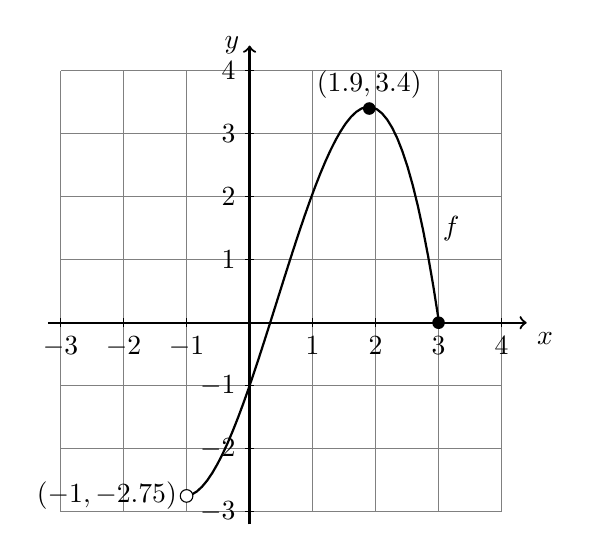
\begin{tikzpicture}[scale=0.8]
        \draw [help lines] (-3,-3) grid (4,4);
        \draw [thick, ->] (-3.2,0) -- (4.4,0) node [below right] {$x$};
        \draw [thick, ->] (0,-3.2)--(0,4.4) node [left] {$y$};
        \foreach \x in {-3,-2,-1,1,2, ...,4} \draw (\x cm,2pt)--(\x cm,-2pt) node[below] {$\x$};
        \foreach \y in {-3,-2,-1,1,2,3,4} \draw (2pt,\y cm)--(-2pt,\y cm) node[left] {$\y$};
        \draw [thick,samples=50,domain=-1:3] plot(\x,-0.5*\x^3+0.65*\x*\x+2.9*\x-1);
        \fill (3,0) circle[radius=0.1];
        \fill (1.9,3.4) circle[radius=0.1] node [above]{$(1.9,3.4)$};
        \node at (3.2,1.5){$f$};
        \fill [white] (-1,-2.75) circle[radius=0.1];
        \draw (-1,-2.75) circle[radius=0.1] node[left]{$(-1,-2.75$)};
      \end{tikzpicture}
    \end{multicols}

\item Part of the function $f(x)=x^3-3x^2-4x+12$ is shown on the graph.
    \begin{center}
    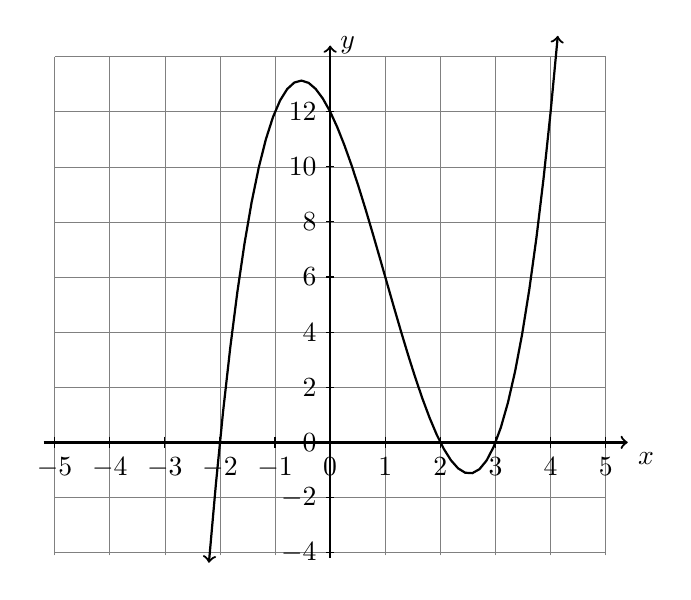
\begin{tikzpicture}[x=1cm, y=0.5cm, scale=0.7]
        \draw [help lines] (-5,-4.1) grid (5,14);
        \draw [thick, ->] (-5.2,0) -- (5.4,0) node [below right] {$x$};
        \draw [thick, ->] (0,-4.2)--(0,14.4) node [right] {$y$};
        \foreach \x in {-5,...,5}
            \draw[shift={(\x,0)}] (0,3pt)--(0,-3pt) node[below] {$\x$};
        \foreach \y in {-4,-2,...,12}
            \draw[shift={(0,\y)}] (2pt,0pt)--(-2pt,0pt) node[left]  {$\y$};
        \draw [<->,thick,samples=50,domain=-2.2:4.13] plot(\x,{(\x)^3-3*(\x)^2-4*(\x)+12});
    \end{tikzpicture}
    \end{center}
    \begin{enumerate}
        \item Write down the $y$-intercept.
        \item Write down the $x$-intercepts.\vspace{0.5cm}
        \item Label the local maximum and local minimum as ordered pairs.
        \item Show that $2$ is an $x$-intercept because $x=2$ is a solution to $f(x)=0$.
    \end{enumerate}

\newpage
\item The rational function $\displaystyle f(x)=\frac{1}{x-1}+3$ and the linear function $\displaystyle g(x)=-\frac{3}{4}x+7$ are graphed below. 
    \begin{multicols}{2}
        \begin{enumerate}
            \item Find the solutions to $f(x)=g(x)$. \vspace{2cm}
            \item Write down the equation of the vertical asymptote to $f$.
        \end{enumerate} \vspace{0.5cm}
        \begin{flushright}
      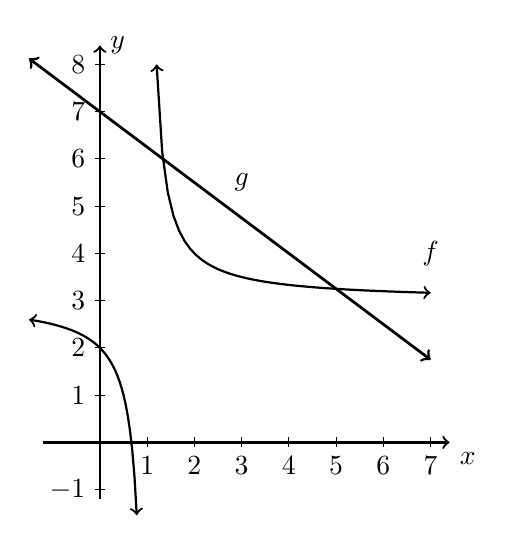
\begin{tikzpicture}[scale=0.6]
        %\draw [help lines] (-3,-3) grid (3,4);
        \draw [thick, ->] (-1.2,0) -- (7.4,0) node [below right] {$x$};
        \draw [thick, ->] (0,-1.2)--(0,8.4) node [right] {$y$};
        \foreach \x in {1,...,7} \draw (\x cm,3pt) -- (\x cm,-3pt) node[anchor=north] {$\x$};
        \foreach \y in {-1,1,2,...,8} \draw (3pt,\y cm) -- (-3pt,\y cm) node[left] {$\y$};
        %\clip (-2,-2) rectangle (6,7);
        \draw [<->,thick,samples=50,domain=1.2:7] plot(\x,{1/(\x-1)+3});
        \draw [<->,thick,samples=50,domain=-1.5:0.78] plot(\x,{1/(\x-1)+3});
        \draw [<->,line width=1.0pt,smooth,samples=20,domain=-1.5:7] plot(\x,-0.75*\x+7);
        \node at (7,4){$f$};
        \node at (3,5.5){$g$};
      \end{tikzpicture}
    \end{flushright}
    \end{multicols}

\item Plot the function $h(x)=x^{3}-4x^{2}-x+4$, labeling the $x-$ and $y$-intercepts. Mark the local maximum and minimums as ordered pairs.
    \begin{center}
        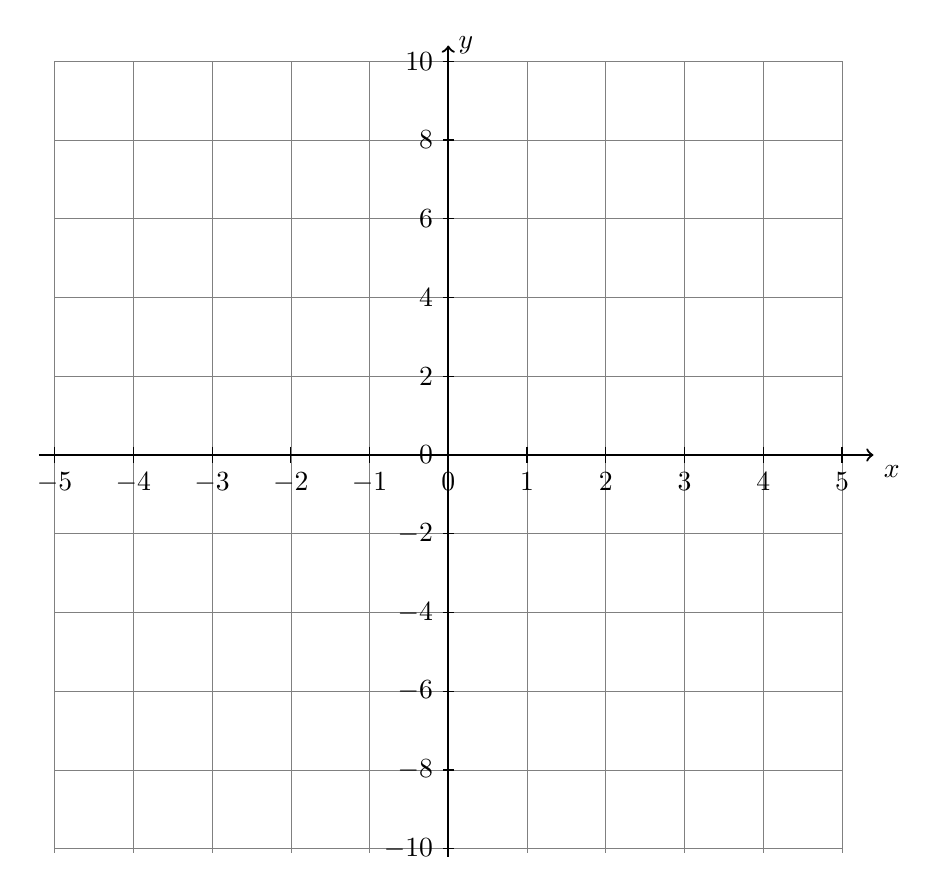
\begin{tikzpicture}[x=1cm, y=0.5cm]
            \draw [help lines] (-5,-10.1) grid (5,10);
            \draw [thick, ->] (-5.2,0) -- (5.4,0) node [below right] {$x$};
            \draw [thick, ->] (0,-10.2)--(0,10.4) node [right] {$y$};
            \foreach \x in {-5,...,5}
                \draw[shift={(\x,0)}] (0,3pt)--(0,-3pt) node[below] {$\x$};
            \foreach \y in {-10,-8,...,10}
                \draw[shift={(0,\y)}] (2pt,0pt)--(-2pt,0pt) node[left]  {$\y$};
            \clip (-5,-10) rectangle (5,10);
            %\draw [<->,thick,smooth,domain=-5:5] plot(\x,{(\x)^3+-4*(\x)^2-1*(\x)+4});
        \end{tikzpicture}
    \end{center}

\end{enumerate}
\end{document}



